% Created 2020-10-05 Mon 11:33
% Intended LaTeX compiler: lualatex
\documentclass[11pt]{article}
\usepackage{graphicx}
\usepackage{grffile}
\usepackage{longtable}
\usepackage{wrapfig}
\usepackage{rotating}
\usepackage[normalem]{ulem}
\usepackage{amsmath}
\usepackage{textcomp}
\usepackage{amssymb}
\usepackage{capt-of}
\usepackage{hyperref}
\usepackage{tabularx}
\usepackage{etoolbox}
\makeatletter
\def\dontdofcolorbox{\renewcommand\fcolorbox[4][]{##4}}
\AtBeginEnvironment{minted}{\dontdofcolorbox}
\makeatother
\usepackage[newfloat]{minted}
\usepackage{amsthm}
\theoremstyle{definition}
\newtheorem{definition}{Definition}[section]
\usepackage{unicode-math}
\usepackage{unicode}
\author{Mark Armstrong}
\date{Fall 2020}
\title{An untyped λ-calculus, \emph{UL}\\\medskip
\large Principles of Programming Languages}
\hypersetup{
   pdfauthor={Mark Armstrong},
   pdftitle={An untyped λ-calculus, \emph{UL}},
   pdfkeywords={},
   pdfsubject={Our first constructed language; a lambda calculus with no type checking (enforcement).},
   pdfcreator={Emacs 27.0.90 (Org mode 9.4)},
   pdflang={English},
   colorlinks,
   linkcolor=blue,
   citecolor=blue,
   urlcolor=blue
   }
\begin{document}

\maketitle

\section{Preamble}
\label{sec:org8a3d65c}
\subsection{{\bfseries\sffamily TODO} Notable references}
\label{sec:orge020f69}
\begin{itemize}
\item Benjamin Pierce,
“\href{https://ebookcentral.proquest.com/lib/mcmu/detail.action?docID=3338823}{Types and Programming Languages}”
\begin{itemize}
\item Chapter 5, The Untyped Lambda-Calculus
\end{itemize}
\end{itemize}

\subsection{{\bfseries\sffamily TODO} Table of contents}
\label{sec:org8e28cbe}
\begin{scriptsize}
\begin{itemize}
\item \hyperref[sec:org8a3d65c]{Preamble}
\end{itemize}
\end{scriptsize}

\section{Introduction}
\label{sec:orgc9a1d1a}
In this section we construct our first simple programming language,
an untyped λ-calculus (lambda calculus).

More specifically, we construct a λ-calculus
without (static) type checking (enforcement),
but including the natural numbers and booleans.

\subsection{What is the λ-calculus?}
\label{sec:org817a8a1}
The λ-calculus is, put simply,
a notation for forming and applying functions.
\begin{itemize}
\item Because the function (procedure, method, subroutine) abstraction
gives us a means of representing control flow,
if we have a means of representing data,
the λ-calculus is a Turing-complete model of computation.
\end{itemize}

\subsection{History}
\label{sec:org61153b8}
The (basic) λ-calculus as we know it was famously invented
by Alonzo Church in the 1920s.
\begin{itemize}
\item This was one culmination of a great deal of work by
mathematicians investigating the foundations of mathematics.
\end{itemize}

As mentioned, the λ-calculus is a Turing-complete model of computation.
\begin{itemize}
\item Other models proposed around the same time include
\begin{itemize}
\item the Turing machine itself (due to Alan Turing), and
\item the general recursive functions (due to Stephen Cole Kleene.)
\end{itemize}
\item Hence the “Church” in the “Church-Turing thesis”.
\end{itemize}

The λ-calculus has since seen widespread use in the study and design
of programming languages.
\begin{itemize}
\item It is useful both as a simple programming language, and
\item as a mathematical object about which statements can be proved.
\end{itemize}

\subsection{Descendents of the λ-calculus}
\label{sec:org3bedc43}
Pure functional programming languages are clearly descended
from the λ-calculus; the λ-calculus embodies their model of computation.
\begin{itemize}
\item Additionally, it is common to have a “lambda” operator
which allows definition of anonymous functions.
\end{itemize}

Imperative languages instead use a model of computation
based on the \emph{Von-Neumann} architecture,
\begin{itemize}
\item which matches our real-world computing devices!
\begin{itemize}
\item Hence imperative languages are naturally lower-level;
one level of abstraction closer to the real computer
that functional languages, which must be translated
to imperative code in order to run.
\end{itemize}
\item This model of computation is a natural extension
of the Turing machine, rather than the λ-calculus
or recursive functions.
\end{itemize}

\section{The basics}
\label{sec:orgd08110a}
In our discussion of abstractions, we mentioned
the abstraction of the function/method/procedure/subroutine.
\begin{itemize}
\item The functional abstraction provides a means
to represent control flow.
\end{itemize}

In its pure version, every term in the λ-calculus
is a function.
\begin{itemize}
\item In order for such a system to be at all useful,
it must of course support higher-order functions;
functions may be applied to functions.
\item Values such as booleans and natural numbers
are \emph{encoded} (represented) by functions.
\end{itemize}

\subsection{The terms}
\label{sec:org4fa43b3}
The pure untyped λ-calculus has just three sort of terms;
\begin{itemize}
\item variables such as \(x\), \(y\), \(z\),
\item \emph{λ-abstractions}, of the form \(λ x → t\),
\begin{itemize}
\item (it is also common to use \(․\) in place of \(→\);
we prefer \(→\) as it emphasises that these are functions)
\item where \(x\) is a variable and \(t\) is a λ-term, and
\end{itemize}
\item applications of the form \(t u\)
\begin{itemize}
\item where \(t\) and \(u\) are λ-terms.
\end{itemize}
\end{itemize}

\subsection{Informal meaning of terms}
\label{sec:orge40ec07}
The meaning of each term is, informally:
\begin{itemize}
\item A λ-abstraction \(λ x → t\) represents a function of one argument,
which, when applied to a term \(u\), substitutes
all free occurrences of \(x\) in \(t\) with \(u\).
\item An application applies the term \(u\) to the function (term) \(t\).
\item A variable on its own (a free variable) has no further meaning.
\begin{itemize}
\item Variables are intended to be \emph{bound}.
\item “Top-level” free variables have no meaning (on their own).
\begin{itemize}
\item Until we construct a new term by λ-abstracting them.
\end{itemize}
\end{itemize}
\end{itemize}

\subsection{Variable binding; free and bound variables}
\label{sec:org4c0ae68}
Recall the notion of free and bound variables.
\begin{itemize}
\item A \emph{variable binder} is an operator which operates on
some number of \emph{variables} as well as \emph{terms}.
\begin{itemize}
\item Examples include quantifiers
such as \(∀\_❙\_•\_\), \(∃\_❙\_•\_\) and \(∑\_❙\_•\_\),
and substitution \(\_[\_→\_]\).
\end{itemize}
\item (For simplicity, let us assume below that variable binders
act on a single variable and a single term.)
\item Let \(B\_•\_\) range over the set of variable binders in a language.
\item An occurrence of a variable \(x\) in a term \(t\) that is \emph{not} in
a subterm of the form \(B x • u\) is called \emph{free}.
\item In a term \(t\) with a subterm of the form \(B x • u\),
all free occurrences of the variable \(x\) that occur within \(u\)
are \emph{bound} by that instance of the binder \(B\).
\begin{itemize}
\item Note: instances of \(x\) which are bound elsewhere are not bound
by that \(B\).
\end{itemize}
\end{itemize}

\subsection{Picturing variable bindings}
\label{sec:org9e40614}
For instance, in the language of predicate logic,
we can view the variables bound like so.
\begin{center}
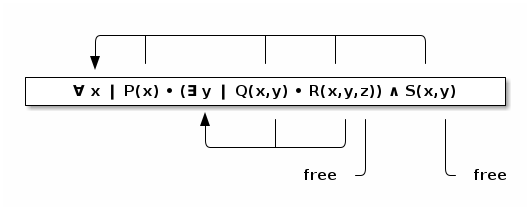
\includegraphics[width=\textwidth]{media/variable-binding.png}
\end{center}

\subsection{Representing functions with multiple arguments}
\label{sec:orgb66067e}
You may have noticed that our method for constructing function
in the λ-calculus (the λ-abstraction)
only allows us to construct single-argument functions.
\begin{itemize}
\item That is, we do not have terms such as \(λ(x,y) → t\).
\item This may seem restrictive,
\item but it turns out to be sufficient.
And it keeps the language simpler theoretically.
\end{itemize}

\subsection{Currying}
\label{sec:orge26f12d}
Rather than complicating our set of terms by admitting
functions of multiple arguments, we use the technique
of \emph{currying} functions.
\begin{itemize}
\item Consider a function \(f : A × B → C\).
\item We can substitute a new function \(f′ : A → (B → C)\)
for \(f\).
\begin{itemize}
\item (By convention, function arrows associate to the right,
so this is equivalent to \(f : A → B → C\).)
\item So \(f′\) is a function which takes an \(A\) and
\emph{produces a function} of type \(B → C\).
\begin{itemize}
\item We usually don't give this new function a name.
\item We can consider this new function as having a \emph{fixed} value
for the \(A\) argument that was provided.
\item (So we must be able to represent higher-order functions
to use Currying.)
\end{itemize}
\end{itemize}
\end{itemize}

\subsection{Examples of λ-terms}
\label{sec:org5c16ce4}
\begin{minted}[breaklines=true]{text}
λ x → x
\end{minted}
is a familiar function; it is the \emph{identity} function.
We will use the name \texttt{id} to refer to this function.

\begin{minted}[breaklines=true]{text}
λ x → λ y → x
\end{minted}

\begin{minted}[breaklines=true]{text}
λ x → λ y → y
\end{minted}

\section{The formal syntax and semantics of \emph{UL}}
\label{sec:org59061b7}
We now discuss the formal semantics of the untyped λ-calculus;
that is, we
\begin{itemize}
\item give a grammar for its syntax, and
\item define operational semantics for the language.
\end{itemize}


\subsection{A grammar for \emph{UL}}
\label{sec:org4e92fec}
\begin{minted}[breaklines=true]{text}
⟨term⟩ ∷= var | λ var → ⟨term⟩ | ⟨term⟩ ⟨term⟩
\end{minted}

In the case that we are restricted to ASCII characters,
we will write abstraction as
\begin{minted}[breaklines=true]{text}
“lambda” var . ⟨term⟩
\end{minted}

\subsection{The operational semantics of \emph{UL}}
\label{sec:org6a42d97}
A term of the form \((λ x → t₁) t₂\) is called a \emph{redex},
meaning \emph{reducible expression}.

The semantics of the λ-calculus is given by a \emph{reduction strategy}
(\emph{β}-reduction strategy);
\begin{itemize}
\item A reduction (β-reduction) transforms a subterm of the form
\begin{itemize}
\item \((λ x → t₁) t₂\) (a redex) to
\item \(t₁[x ≔ t₂]\).
\begin{itemize}
\item (There are various syntactic representations of substitutions;
we prefer to the substitution operation to come after the term
where the substitution is carried out (\(t₁\)), and to use
the “becomes” operator to imply free instance of \(x\) become \(t₂\).
\item Pierce instead uses the form \([x ↦ t₂]t₁\), with the
substitution operation coming before the term,
and using the “maps to” operator instead of “becomes”.
\item You may also see forms such as \([x\backslash t₁]\) or \([t₁/x]\).)
\end{itemize}
\end{itemize}
\end{itemize}

\subsection{Reduction strategies}
\label{sec:org5f1c31e}
Given an arbitrary term, there may be several subterms which are redexes,
\begin{itemize}
\item so we have a choice of what subterm to reduce.
\end{itemize}
A reduction strategy limits our choice of which redex to reduce.

Several strategies have been studied. We discuss just four of them.
\begin{itemize}
\item full β-reduction,
\item normal order,
\item call by name, and
\item call by value.
\end{itemize}
We only give a full formal treatment to call-by-value.

The last two you may know as names of parameter passing methods
from (practical) programming languages.
\begin{itemize}
\item There is a direct correspondance between reduction strategies
and parameter passing methods.
\end{itemize}

\subsection{Reduction strategies: full β-reduction and normal order}
\label{sec:orga435b41}
The \emph{full β-reduction} strategy is, essentially, to have no
strategy at all.

Under full β-reduction, and redex can be reduced at any point.

The \emph{normal order} strategy enforces that the
leftmost, outermost redex is always reduced first.

\subsection{Reduction strategies: call by name and call by value}
\label{sec:orgf76a00f}
The \emph{call by name} strategy builds on the normal order strategy
\begin{itemize}
\item by mandating that no reductions take place inside abstractions.
\item So “arguments cannot be evaluated before being applied”.
\end{itemize}

The \emph{call by value} strategy also builds on the normal order strategy,
\begin{itemize}
\item by mandating that a redex is reduced only when its right hand side
\begin{itemize}
\item (the “argument”)
\end{itemize}
cannot be reduced (is a value.)
\end{itemize}

\subsection{A formal description of call by value semantics}
\label{sec:org792090e}

Let us use the convention that variable names involving
\begin{itemize}
\item \texttt{t} represent arbitrary λ-terms, whereas variable names involving
\item \texttt{v} represent irreducible λ-terms (values).
\end{itemize}

Then we may give a formal description of call-by-value semantics
using inference rules.
\begin{minted}[breaklines=true]{text}
   t₁ ⟶ t₁′
–––––––––––––––– Applicationˡ
t₁ t₂ ⟶ t₁′ t₂


   
   t₂ ⟶ t₂′
–––––––––––––––– Applicationʳ
v₁ t₂ ⟶ v₁ t₂′


   
–––––––––––––––––––––––– Application to abstraction
(λ x → t) v ⟶ t[x ≔ v]
\end{minted}

\subsection{α-conversion and η-conversion}
\label{sec:org37e8773}
:TODO:


β-reduction gives us one way to equate terms;
\begin{itemize}
\item two terms “have the same value” if they both reduce to the same
value (irreducible term.)
\end{itemize}

:TODO:

\subsection{Normalisation}
\label{sec:orgb5accb7}

A λ-term is said to be in \emph{normal form} if it cannot be reduced.

:TODO:

\section{λ-encodings}
\label{sec:org69b1c42}
As mentioned previously, in the pure λ-calculus,
every term is a function.
\begin{itemize}
\item There are no basic types of data.
\end{itemize}

So, we must have a way of representing any data as
a function.
\begin{itemize}
\item We call these Church encodings.
\end{itemize}

We will show how to do this for
\begin{itemize}
\item booleans,
\item pairs, and
\item natural numbers,
\end{itemize}
and give some “combinators” which operate on these kinds of data.

\subsection{Church booleans}
\label{sec:orgdc36ca5}

We define the following terms to represent boolean values.
\begin{itemize}
\item \texttt{tru} represents truth, and
\item \texttt{fls} represents false.
\end{itemize}
\begin{minted}[breaklines=true]{text}
tru = λ t → λ f → t
fls = λ t → λ f → f
\end{minted}

These choices are \emph{somewhat} arbitrary.
\begin{itemize}
\item We could choose any two distinct λ-terms.
\item But they are not really arbitrary;
these two terms embody the idea that a boolean value
is a “choice” between two options.
\begin{itemize}
\item \texttt{tru}, when given two arguments, “chooses” the first.
\item \texttt{fls}, when given two arguments, “chooses” the second.
\end{itemize}
\end{itemize}

\subsection{Defining \texttt{if-then-else} using Church booleans}
\label{sec:org5be900c}

Since the Church encoded booleans already “perform” a choice,
defining an “\texttt{if-then-else}” construct
using them is quite straightforward.
\begin{minted}[breaklines=true]{text}
test = λ l → λ m → λ n → l m n
\end{minted}
The intention is that
\begin{itemize}
\item the first argument is a Church boolean,
\item the second is the “\texttt{then}” branch, and
\item the third is the “\texttt{else}” branch.
\end{itemize}

Notice that \texttt{test b v w} simply reduces to \texttt{b v w};
\begin{itemize}
\item the boolean \texttt{b} really “does the work”
of choosing between \texttt{v} and \texttt{w}.
\end{itemize}

\subsection{Pairs}
\label{sec:org6a31c37}

:TODO:

\subsection{Church numerals}
\label{sec:org07fd557}

:TODO:

\subsection{Addition and multiplication}
\label{sec:org84be5db}

:TODO:

\section{Enriching the calculus}
\label{sec:org365888d}

\section{}
\label{sec:org849d607}
\end{document}
